\chapter{Appendix A: Core Source Code Implementations}

\section*{A.1 Go Backend: Asynchronous Worker Pool Implementation}
The following Go snippet illustrates the core logic of the worker pool responsible for managing long-running LLM inference tasks asynchronously, ensuring the main HTTP thread remains unblocked.

\begin{lstlisting}[caption=Worker Pool implementation in Go]
package worker

import (
	"context"
	"log"
	"sync"
)

// Job represents a generation task requested by a user
type Job struct {
	ID        string
	Payload   string
	JobType   string // "summary", "quiz", "flashcard"
	UserID    string
}

// WorkerPool manages a pool of goroutines for processing LLM jobs
type WorkerPool struct {
	concurrency int
	jobQueue    chan Job
	wg          sync.WaitGroup
}

func NewWorkerPool(concurrency int) *WorkerPool {
	return &WorkerPool{
		concurrency: concurrency,
		jobQueue:    make(chan Job, 100),
	}
}

func (wp *WorkerPool) Start(ctx context.Context) {
	for i := 0; i < wp.concurrency; i++ {
		wp.wg.Add(1)
		go wp.worker(ctx, i)
	}
}

func (wp *WorkerPool) worker(ctx context.Context, id int) {
	defer wp.wg.Done()
	for {
		select {
		case <-ctx.Done():
			log.Printf("Worker %d shutting down", id)
			return
		case job := <-wp.jobQueue:
			log.Printf("Worker %d processing job %s", id, job.ID)
			processLLMTask(job) // Calls Gemini API and saves to DB
		}
	}
}

func (wp *WorkerPool) Submit(job Job) {
	wp.jobQueue <- job
}
\end{lstlisting}

\section*{A.2 React Frontend: Custom WebSocket Hook}
This custom React hook demonstrates how the frontend establishes a persistent WebSocket connection to receive real-time updates regarding AI generation job statuses without polling.

\begin{lstlisting}[caption=React WebSocket Hook]
import { useEffect, useState } from 'react';

export function useJobSocket(jobId) {
    const [status, setStatus] = useState('pending');
    const [progress, setProgress] = useState(0);

    useEffect(() => {
        if (!jobId) return;
        const ws = new WebSocket(`ws://localhost:8080/ws/jobs/${jobId}`);
        
        ws.onmessage = (event) => {
            const data = JSON.parse(event.data);
            setStatus(data.status);
            setProgress(data.progress || 0);
            
            if (data.status === 'completed' || data.status === 'failed') {
                ws.close();
            }
        };

        return () => ws.close();
    }, [jobId]);

    return { status, progress };
}
\end{lstlisting}

\chapter{Appendix B: API and Data Structures}

\section*{B.1 RESTful API Endpoints}
The following table outlines the primary REST API endpoints exposed by the Go backend.

\begin{table}[h]
\centering
\begin{tabular}{|l|l|l|}
\hline
\textbf{Method} & \textbf{Endpoint} & \textbf{Description} \\ \hline
POST & \texttt{/api/v1/auth/login} & Authenticates user and returns JWT \\ \hline
POST & \texttt{/api/v1/content/upload} & Uploads PDF/Video URL for processing \\ \hline
GET  & \texttt{/api/v1/content/\{id\}} & Retrieves generated study materials \\ \hline
GET  & \texttt{/api/v1/flashcards/review} & Fetches due flashcards using SRS logic \\ \hline
POST & \texttt{/api/v1/flashcards/\{id\}/grade} & Submits spaced repetition score (1-5) \\ \hline
\end{tabular}
\caption{Core API endpoints of the Lectura platform.}
\end{table}

\section*{B.2 LLM JSON Response Schema}
When generating quizzes, the system forces the LLM to return a strict JSON structure. Below is an example of the validated output schema for multiple-choice questions.

\begin{lstlisting}[caption=LLM Quiz Response Schema]
{
  "quiz_id": "qz_987654321",
  "topic": "Neural Networks",
  "questions": [
    {
      "question_text": "What is the primary function of an activation function?",
      "options": [
        "To initialize weights",
        "To introduce non-linearity into the network",
        "To calculate the loss",
        "To perform backpropagation"
      ],
      "correct_answer_index": 1,
      "explanation": "Activation functions introduce non-linear properties..."
    }
  ]
}
\end{lstlisting}

\chapter{Appendix C: User Manual and Interface Guide}

\section*{C.1 System Dashboard}
Upon successful authentication, users are greeted by the main dashboard. This interface provides a holistic overview of their academic progress, including recently processed documents, upcoming flashcard reviews due today, and overall study statistics.
\begin{figure}[htbp]
\centering

\includegraphics[width=0.8\textwidth]{chapters/chapter07/images/dashboard.png}
\caption{User Dashboard illustrating active learning metrics.}
\end{figure}

\section*{C.2 Material Generation and Interaction}
To process new material, the user clicks "New Document" and provides a YouTube URL, PDF, or raw text. Once processing completes, the platform presents a unified learning view. The "Summary" tab presents structured Cornell notes.
\begin{figure}[htbp]
\centering
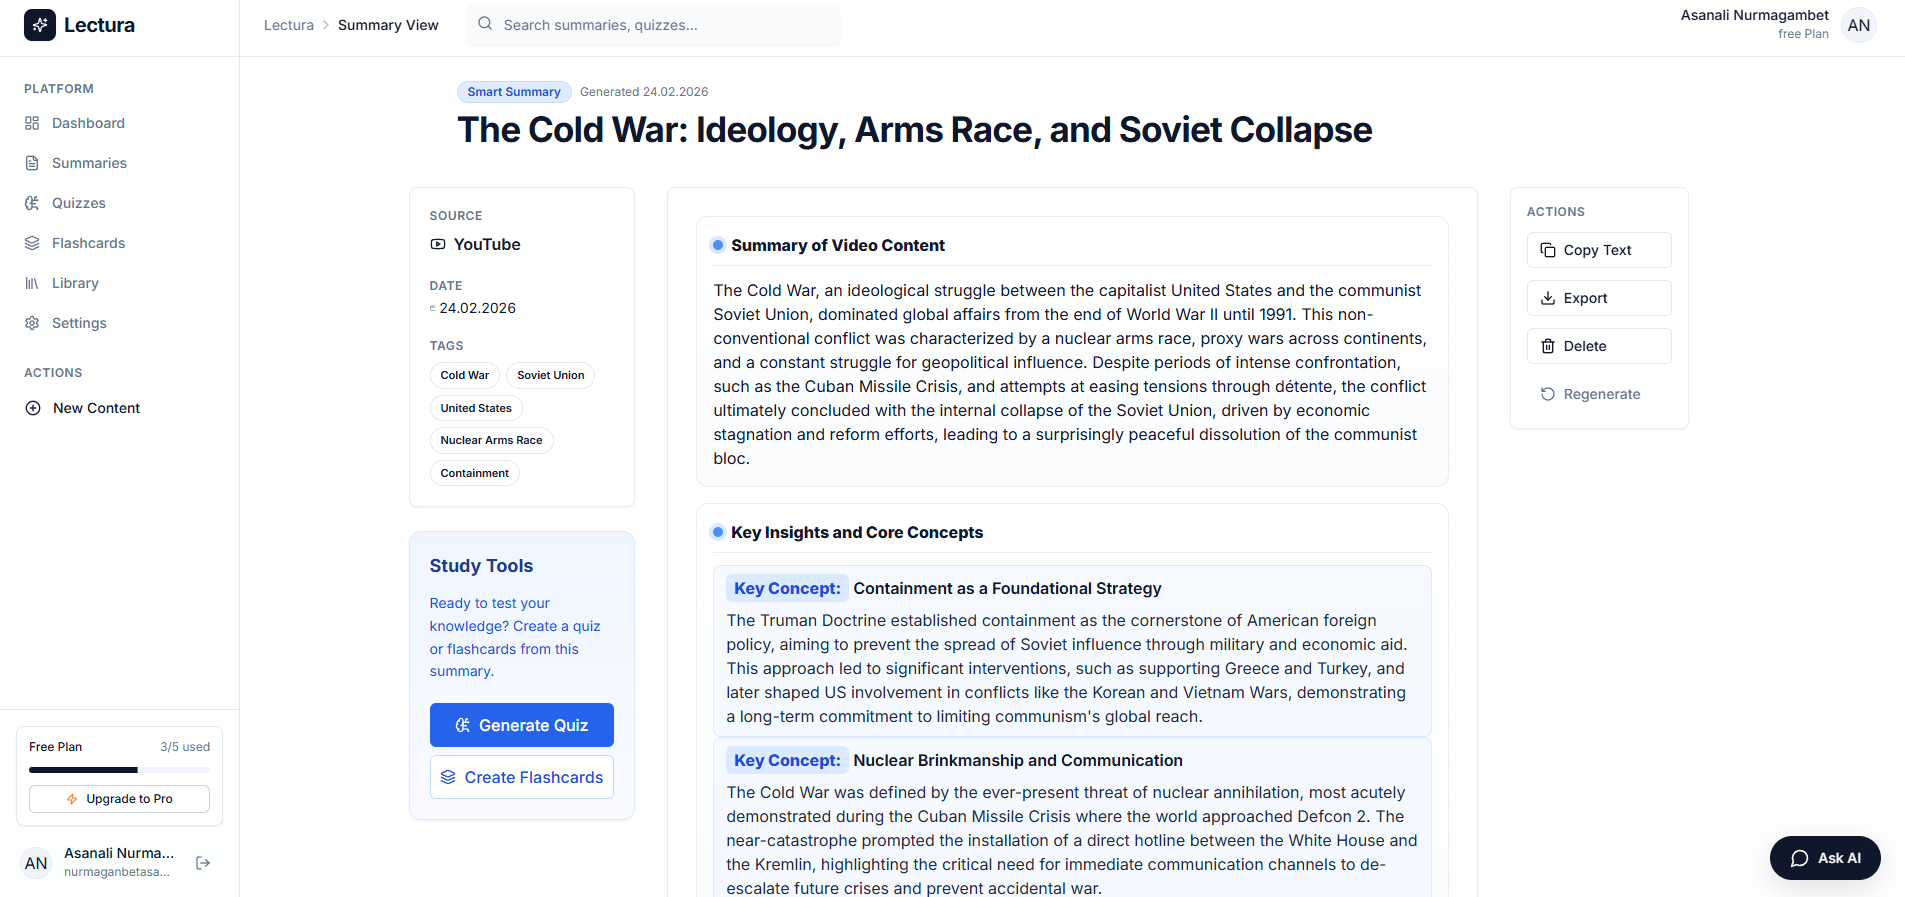
\includegraphics[width=0.8\textwidth]{chapters/chapter07/images/summary.png}
\caption{Generated summary using the Cornell Note-taking format.}
\end{figure}

\section*{C.3 Spaced Repetition Flashcards}
The "Flashcards" tab isolates key concepts and vocabulary. Users flip the card to reveal the answer and rate their recall difficulty (e.g., Easy, Good, Hard, Again). The backend's SRS algorithm uses these ratings to schedule the next review.
\begin{figure}[htbp]
\centering
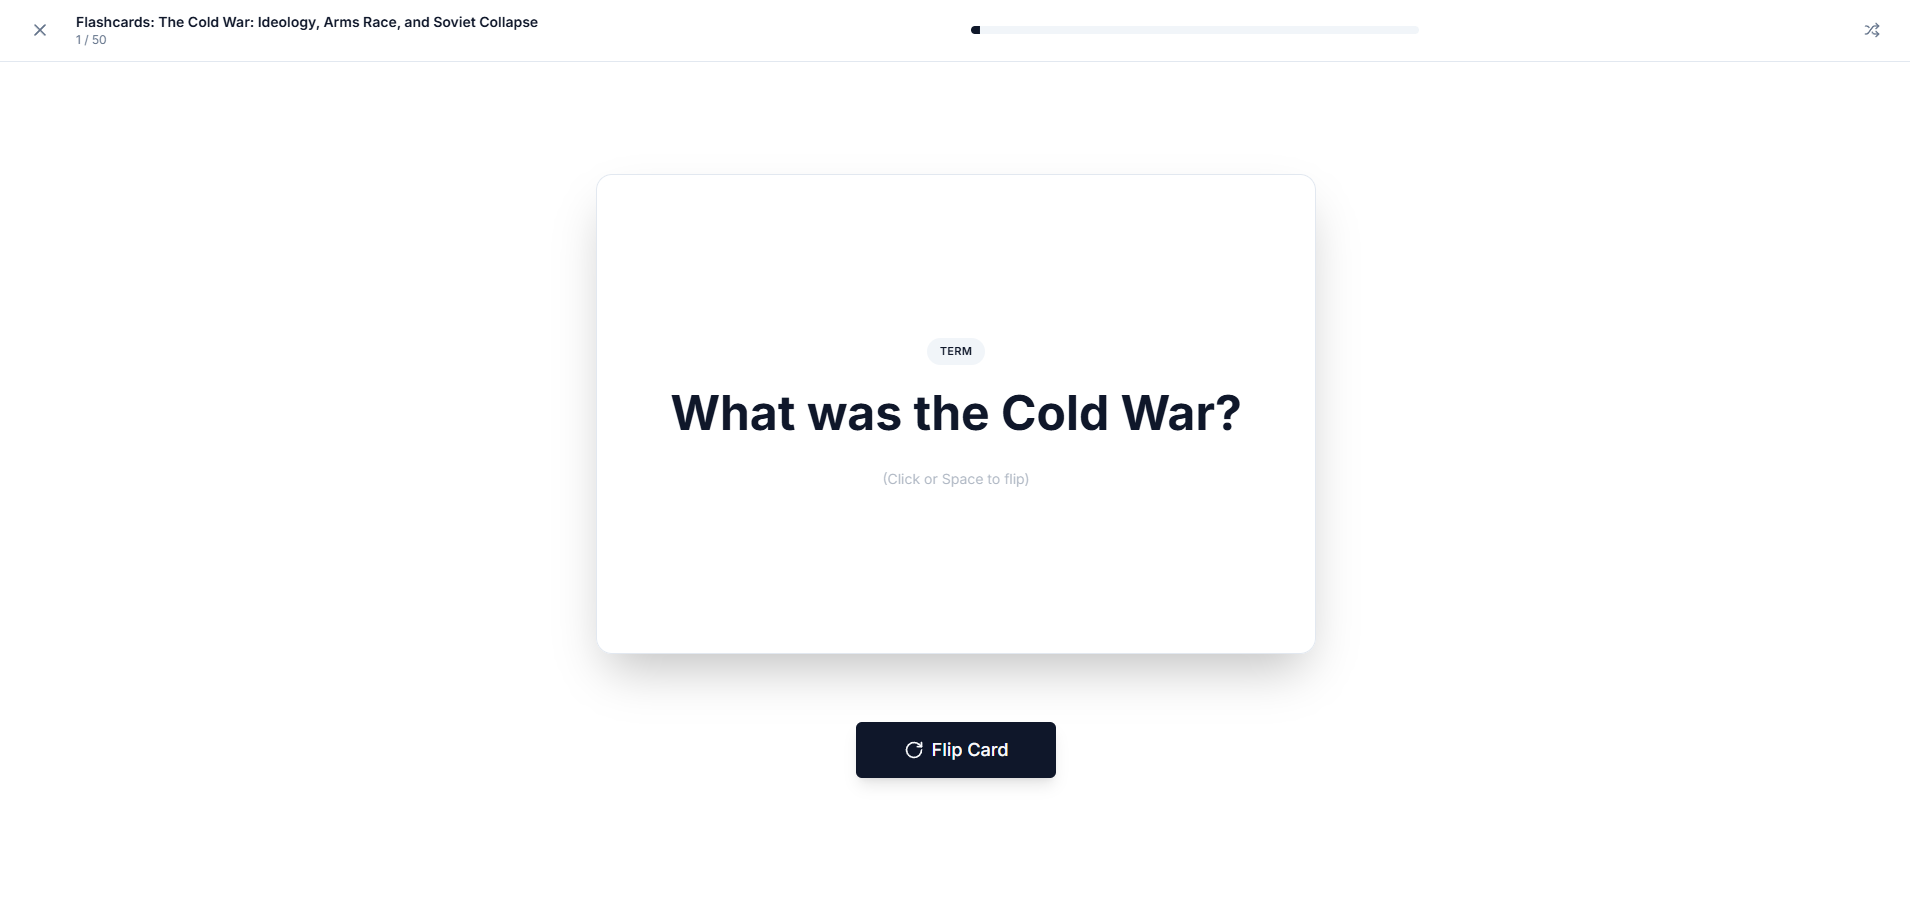
\includegraphics[width=0.8\textwidth]{chapters/chapter07/images/flashcards.png}
\caption{Interactive flashcard interface with spaced repetition grading.}
\end{figure}

\chapter{Appendix D: User Acceptance Testing Questionnaire}
The following questions were distributed to 20 university students during the User Acceptance Testing (UAT) phase. Responses were collected on a 5-point Likert scale (1 = Strongly Disagree, 5 = Strongly Agree).

\begin{enumerate}
    \item Usability: The user interface is intuitive and easy to navigate without prior training.
    \item Accuracy: The AI-generated summaries accurately capture the main points of the uploaded lectures or documents.
    \item Quality of Assessment: The multiple-choice quizzes are relevant and distractors (wrong answers) are pedagogically plausible.
    \item Effectiveness: The spaced repetition flashcards helped me memorize terminology faster than traditional manual note-taking.
    \item Time Savings: Using the platform significantly reduced the time I spend preparing study materials for exams.
    \item Performance: The application is responsive, and generation waiting times are acceptable.
    \item Overall Satisfaction: I would recommend this platform to my classmates as a primary study tool.
\end{enumerate}
